\section{三重积分}

\begin{problem}{三重积分计算}{Triple-Integral-Calculation}
    计算下列三重积分：
    \begin{enumerate}
        \item $\iiint_V xy \d x \d y \d z$，$V: 1 \le x \le 2, -2 \le y \le 1, 0 \le z \le \frac{1}{2}$；
        \item $\iiint_V xy^2 z^3 \d x \d y \d z$，$V$：由 $z = xy, y = x, x = 1, z = 0$ 围成；
        \item $\iiint_V y \cos(x + z) \d x \d y \d z$，$V$：由 $y = \sqrt{x}, y = 0, z = 0, x + z = \frac{\uppi}{2}$ 围成；
        \item $\iiint_V (a - y) \d x \d y \d z$，$V$：由 $y = 0, z = 0, 2x + y = a, x + y = a, y + z = a$ 围成。
    \end{enumerate}
\end{problem}

\begin{solution}
    \ansitem{1}
    由于积分区域 $V$ 为长方体域，且被积函数关于变量可分离，积分可写作
    \begin{equation}
        \begin{aligned}
            I & = \int_1^2 x \d x \int_{-2}^1 y \d y \int_0^{1/2} \d z                                                        \\
              & = \left[ \frac{1}{2}x^2 \right]_1^2 \cdot \left[ \frac{1}{2}y^2 \right]_{-2}^1 \cdot \left[ z \right]_0^{1/2} \\
              & = \left( 2 - \frac{1}{2} \right) \cdot \left( \frac{1}{2} - 2 \right) \cdot \frac{1}{2}                       \\
              & = \frac{3}{2} \cdot \left( -\frac{3}{2} \right) \cdot \frac{1}{2}.
        \end{aligned}
    \end{equation}
    \begin{equation}
        \iiint_V xy \d x \d y \d z = \boxed{-\frac{9}{8}}
    \end{equation}

    \ansitem{2}
    积分区域 $V$ 可表示为 $0 \le x \le 1, 0 \le y \le x, 0 \le z \le xy$，则有
    \begin{equation}
        \begin{aligned}
            I & = \int_0^1 \d x \int_0^x \d y \int_0^{xy} xy^2 z^3 \d z                   \\
              & = \int_0^1 x \d x \int_0^x y^2 \left[ \frac{1}{4} z^4 \right]_0^{xy} \d y \\
              & = \frac{1}{4} \int_0^1 x^5 \d x \int_0^x y^6 \d y                         \\
              & = \frac{1}{4} \int_0^1 x^5 \cdot \frac{1}{7} x^7 \d x.
        \end{aligned}
    \end{equation}
    计算定积分可得
    \begin{equation}
        \iiint_V xy^2 z^3 \d x \d y \d z = \boxed{\frac{1}{364}}
    \end{equation}

    \ansitem{3}
    积分区域 $V$ 在 $xz$ 平面上的投影域 $D_{xz}$ 由 $x=0, z=0, x+z=\frac{\uppi}{2}$ 围成，对于 $D_{xz}$ 内任意一点，变量 $y$ 的范围为 $0 \le y \le \sqrt{x}$，故
    \begin{equation}
        \begin{aligned}
            I & = \int_0^{\uppi/2} \d x \int_0^{\uppi/2 - x} \d z \int_0^{\sqrt{x}} y \cos(x + z) \d y \\
              & = \int_0^{\uppi/2} \d x \int_0^{\uppi/2 - x} \frac{1}{2}x \cos(x + z) \d z             \\
              & = \frac{1}{2} \int_0^{\uppi/2} x \left[ \sin(x + z) \right]_0^{\uppi/2 - x} \d x       \\
              & = \frac{1}{2} \int_0^{\uppi/2} x (1 - \sin x) \d x.
        \end{aligned}
    \end{equation}
    利用分部积分法，可知 $\int_0^{\uppi/2} x \sin x \d x = 1$，则
    \begin{equation}
        \iiint_V y \cos(x + z) \d x \d y \d z = \boxed{\frac{\uppi^2}{16} - \frac{1}{2}}
    \end{equation}

    \ansitem{4}
    由边界条件可知，对于固定的 $y \in [0, a]$，截面区域在 $xz$ 平面上满足 $0 \le z \le a - y$ 且 $\frac{a-y}{2} \le x \le a - y$。积分计算如下
    \begin{equation}
        \begin{aligned}
            I & = \int_0^a \d y \int_{(a-y)/2}^{a-y} \d x \int_0^{a-y} (a-y) \d z \\
              & = \int_0^a (a-y) \d y \int_{(a-y)/2}^{a-y} (a-y) \d x             \\
              & = \int_0^a (a-y)^2 \left( (a-y) - \frac{a-y}{2} \right) \d y      \\
              & = \frac{1}{2} \int_0^a (a-y)^3 \d y.
        \end{aligned}
    \end{equation}
    令 $u = a - y$，则
    \begin{equation}
        \iiint_V (a - y) \d x \d y \d z = \boxed{\frac{a^4}{8}}
    \end{equation}
\end{solution}

\begin{problem}{三重积分计算}{Triple-Integral-Calculation-2}
    计算下列积分值：
    \begin{enumerate}
        \item $\int_{0}^{2} \d x \int_{0}^{\sqrt{2x-x^{2}}} \d y \int_{0}^{a} z \sqrt{x^{2}+y^{2}} \d z$；
        \item $\int_{-R}^{R} \d x \int_{-\sqrt{R^{2}-x^{2}}}^{\sqrt{R^{2}-x^{2}}} \d y \int_{0}^{\sqrt{R^{2}-x^{2}-y^{2}}} (x^{2}+y^{2}) \d z$；
        \item $\int_{0}^{1} \d x \int_{0}^{\sqrt{1-x^{2}}} \d y \int_{0}^{\sqrt{1-x^{2}-y^{2}}} \sqrt{x^{2}+y^{2}+z^{2}} \d z$；
        \item $\int_{0}^{1} \d x \int_{0}^{\sqrt{1-x^{2}}} \d y \int_{\sqrt{x^{2}+y^{2}}}^{\sqrt{2-x^{2}-y^{2}}} z^{2} \d z$。
    \end{enumerate}
\end{problem}

\begin{solution}
    \ansitem{1}
    积分区域在 $xy$ 平面上的投影为 $D = \{(x, y) \mid 0 \le x \le 2, 0 \le y \le \sqrt{2x-x^{2}}\}$，这是一个半圆 $(x-1)^{2} + y^{2} \le 1$ ($y \ge 0$)。采用柱面坐标，有 $x = r \cos \theta, y = r \sin \theta$，其边界为 $r = 2 \cos \theta$，范围为 $\theta \in [0, \uppi/2], r \in [0, 2\cos \theta]$。
    \begin{equation}
        \begin{aligned}
            \text{原式} & = \int_{0}^{\uppi/2} \d \theta \int_{0}^{2\cos \theta} r \d r \int_{0}^{a} z \cdot r \d z \\
                      & = \frac{a^{2}}{2} \int_{0}^{\uppi/2} \d \theta \int_{0}^{2\cos \theta} r^{2} \d r         \\
                      & = \frac{4 a^{2}}{3} \int_{0}^{\uppi/2} \cos^{3} \theta \d \theta                          \\
                      & = \frac{4 a^{2}}{3} \cdot \frac{2}{3} \label{eq:integral-1}
        \end{aligned}
    \end{equation}
    \begin{equation}
        I = \boxed{\frac{8a^{2}}{9}}
    \end{equation}

    \ansitem{2}
    积分区域为上半球体 $x^{2} + y^{2} + z^{2} \le R^{2}$ ($z \ge 0$)。采用柱面坐标，有 $x^{2} + y^{2} = r^{2}$，区域表示为 $0 \le \theta \le 2\uppi, 0 \le r \le R, 0 \le z \le \sqrt{R^{2}-r^{2}}$。
    \begin{equation}
        \begin{aligned}
            \text{原式} & = \int_{0}^{2\uppi} \d \theta \int_{0}^{R} r \d r \int_{0}^{\sqrt{R^{2}-r^{2}}} r^{2} \d z \\
                      & = 2\uppi \int_{0}^{R} r^{3} \sqrt{R^{2}-r^{2}} \d r \label{eq:integral-2}
        \end{aligned}
    \end{equation}
    令 $u = \sqrt{R^{2}-r^{2}}$，则 $r^{2} = R^{2}-u^{2}, r \d r = -u \d u$。
    \begin{equation}
        \begin{aligned}
            \text{原式} & = 2\uppi \int_{R}^{0} (R^{2}-u^{2}) \cdot u \cdot (-u) \d u   \\
                      & = 2\uppi \int_{0}^{R} (R^{2}u^{2} - u^{4}) \d u               \\
                      & = 2\uppi \left[ \frac{1}{3} R^{5} - \frac{1}{5} R^{5} \right]
        \end{aligned}
    \end{equation}
    \begin{equation}
        I = \boxed{\frac{4\uppi R^{5}}{15}}
    \end{equation}

    \ansitem{3}
    积分区域为单位球在第一卦限的部分。采用球面坐标，有 $0 \le \rho \le 1, 0 \le \theta \le \uppi/2, 0 \le \varphi \le \uppi/2$。
    \begin{equation}
        \begin{aligned}
            \text{原式} & = \int_{0}^{\uppi/2} \d \theta \int_{0}^{\uppi/2} \sin \varphi \d \varphi \int_{0}^{1} \rho \cdot \rho^{2} \d \rho                         \\
                      & = \frac{\uppi}{2} \cdot \left[ -\cos \varphi \right]_{0}^{\uppi/2} \cdot \left[ \frac{1}{4} \rho^{4} \right]_{0}^{1} \label{eq:integral-3}
        \end{aligned}
    \end{equation}
    \begin{equation}
        I = \boxed{\frac{\uppi}{8}}
    \end{equation}

    \ansitem{4}
    积分区域由锥面 $z = \sqrt{x^{2}+y^{2}}$ 与球面 $x^{2}+y^{2}+z^{2} = 2$ 在第一卦限围成。采用球面坐标，锥面对应 $\varphi = \uppi/4$，球面对应 $\rho = \sqrt{2}$。区域为 $0 \le \theta \le \uppi/2, 0 \le \varphi \le \uppi/4, 0 \le \rho \le \sqrt{2}$。
    \begin{equation}
        \begin{aligned}
            \text{原式} & = \int_{0}^{\uppi/2} \d \theta \int_{0}^{\uppi/4} \d \varphi \int_{0}^{\sqrt{2}} (\rho \cos \varphi)^{2} \cdot \rho^{2} \sin \varphi \d \rho \\
                      & = \frac{\uppi}{2} \int_{0}^{\uppi/4} \cos^{2} \varphi \sin \varphi \d \varphi \int_{0}^{\sqrt{2}} \rho^{4} \d \rho                           \\
                      & = \frac{\uppi}{2} \cdot \left[ -\frac{1}{3} \cos^{3} \varphi \right]_{0}^{\uppi/4} \cdot \frac{4\sqrt{2}}{5}                                 \\
                      & = \frac{\uppi}{2} \cdot \frac{1}{3} \left( 1 - \frac{\sqrt{2}}{4} \right) \cdot \frac{4\sqrt{2}}{5} \label{eq:integral-4}
        \end{aligned}
    \end{equation}
    \begin{equation}
        I = \boxed{\frac{(2\sqrt{2}-1)\uppi}{15}}
    \end{equation}
\end{solution}

\begin{problem}{三重积分计算}{Triple-Integrals}
    计算下列三重积分：
    \begin{enumerate}
        \item $\iiint_{V}\left(x^{2}+y^{2}\right) \d x \d y \d z$，其中 $V$ 是由 $x^{2}+y^{2}=2 z$ 与 $z=2$ 围成的区域；
        \item $\iiint_{V} \sqrt{x^{2}+y^{2}} \d x \d y \d z$，其中 $V$ 是由 $x^{2}+y^{2}=z^{2}$ 与 $z=1$ 围成的区域；
        \item $\iiint_{V} z \d x \d y \d z$，其中 $V$ 是由 $\sqrt{4-x^{2}-y^{2}}=z$ 与 $x^{2}+y^{2}=3 z$ 围成的区域；
        \item $\iiint_{V} x y z \d x \d y \d z$，其中 $V$ 是 $x^{2}+y^{2}+z^{2} \leqslant 1$ 的第一卦限部分；
        \item $\iiint_{V} x^{2} \d x \d y \d z$，其中 $V$ 是由曲面 $z=y^{2}$、$z=4 y^{2}(y>0)$ 及平面 $z=x$、$z=2 x$、$z=1$ 所围成的区域；
        \item $\iiint_{V}\left|x^{2}+y^{2}+z^{2}-1\right| \d x \d y \d z$，其中 $V: x^{2}+y^{2}+z^{2} \leqslant 4$；
        \item $\iiint_{V} \e^{|z|} \d x \d y \d z$，其中 $V: x^{2}+y^{2}+z^{2} \leqslant 1$；
        \item $\iiint_{V}(|x|+z) \e^{-\left(x^{2}+y^{2}+z^{2}\right)} \d x \d y \d z$，其中 $V: 1 \leqslant x^{2}+y^{2}+z^{2} \leqslant 4$。
    \end{enumerate}
\end{problem}

\begin{solution}
    \ansitem{1}
    采用柱面坐标，令 $x=\rho \cos \theta$、$y=\rho \sin \theta$、$z=z$。积分区域 $V$ 可表示为 $0 \leqslant \theta \leqslant 2 \uppi$、$0 \leqslant z \leqslant 2$、$0 \leqslant \rho \leqslant \sqrt{2 z}$。

    \begin{equation}
        \begin{aligned}
            \iiint_{V}\left(x^{2}+y^{2}\right) \d x \d y \d z & = \int_{0}^{2 \uppi} \d \theta \int_{0}^{2} \d z \int_{0}^{\sqrt{2 z}} \rho^{2} \cdot \rho \d \rho \\
                                                              & = 2 \uppi \int_{0}^{2} \left[ \frac{1}{4} \rho^{4} \right]_{0}^{\sqrt{2 z}} \d z                   \\
                                                              & = \frac{\uppi}{2} \int_{0}^{2} (2 z)^{2} \d z                                                      \\
                                                              & = 2 \uppi \left[ \frac{1}{3} z^3 \right]_{0}^{2}                                                   \\
                                                              & = \frac{16 \uppi}{3} \label{eq:I1}
        \end{aligned}
    \end{equation}

    \begin{equation}
        I = \boxed{\frac{16 \uppi}{3}}
    \end{equation}

    \ansitem{2}
    采用柱面坐标，积分区域 $V$ 可表示为 $0 \leqslant \theta \leqslant 2 \uppi$、$0 \leqslant z \leqslant 1$、$0 \leqslant \rho \leqslant z$。

    \begin{equation}
        \begin{aligned}
            \iiint_{V} \sqrt{x^{2}+y^{2}} \d x \d y \d z & = \int_{0}^{2 \uppi} \d \theta \int_{0}^{1} \d z \int_{0}^{z} \rho \cdot \rho \d \rho \\
                                                         & = 2 \uppi \int_{0}^{1} \frac{1}{3} z^{3} \d z                                         \\
                                                         & = 2 \uppi \cdot \frac{1}{12}                                                          \\
                                                         & = \frac{\uppi}{6} \label{eq:I2}
        \end{aligned}
    \end{equation}

    \begin{equation}
        I = \boxed{\frac{\uppi}{6}}
    \end{equation}

    \ansitem{3}
    联立方程 $\sqrt{4-x^{2}-y^{2}}=z$ 与 $x^{2}+y^{2}=3 z$。由于 $z \geqslant 0$，解得交线位于 $z=1$ 平面处。积分区域在 $xy$ 平面上的投影为圆盘 $D: x^2+y^2 \leqslant 3$。

    \begin{equation}
        \begin{aligned}
            \iiint_{V} z \d x \d y \d z & = \iint_{D} \d x \d y \int_{\frac{x^2+y^2}{3}}^{\sqrt{4-x^2-y^2}} z \d z                                                 \\
                                        & = \frac{1}{2} \iint_{D} \left( 4 - (x^2 + y^2) - \frac{(x^2+y^2)^2}{9} \right) \d x \d y                                 \\
                                        & = \frac{1}{2} \int_{0}^{2 \uppi} \d \theta \int_{0}^{\sqrt{3}} \left( 4 - \rho^2 - \frac{\rho^4}{9} \right) \rho \d \rho \\
                                        & = \uppi \left[ 2 \rho^2 - \frac{1}{4} \rho^4 - \frac{1}{54} \rho^6 \right]_{0}^{\sqrt{3}}                                \\
                                        & = \uppi \left( 6 - \frac{9}{4} - \frac{1}{2} \right) \label{eq:I3}
        \end{aligned}
    \end{equation}

    \begin{equation}
        I = \boxed{\frac{13 \uppi}{4}}
    \end{equation}

    \ansitem{4}
    采用球坐标，积分区域 $V$ 对应的参数范围为 $0 \leqslant r \leqslant 1$、$0 \leqslant \theta \leqslant \frac{\uppi}{2}$、$0 \leqslant \varphi \leqslant \frac{\uppi}{2}$。

    \begin{equation}
        \begin{aligned}
            \iiint_{V} x y z \d x \d y \d z & = \int_{0}^{\frac{\uppi}{2}} \sin \theta \cos \theta \d \theta \int_{0}^{\frac{\uppi}{2}} \sin^3 \varphi \cos \varphi \d \varphi \int_{0}^{1} r^5 \d r   \\
                                            & = \left[ \frac{1}{2} \sin^2 \theta \right]_{0}^{\frac{\uppi}{2}} \cdot \left[ \frac{1}{4} \sin^4 \varphi \right]_{0}^{\frac{\uppi}{2}} \cdot \frac{1}{6} \\
                                            & = \frac{1}{2} \cdot \frac{1}{4} \cdot \frac{1}{6} \label{eq:I4}
        \end{aligned}
    \end{equation}

    \begin{equation}
        I = \boxed{\frac{1}{48}}
    \end{equation}

    \ansitem{5}
    根据围成区域的曲面方程，选取积分顺序。对于固定的 $z \in [0, 1]$，区域的截面范围为 $x \in [\frac{z}{2}, z]$ 及 $y \in [\frac{\sqrt{z}}{2}, \sqrt{z}]$。

    \begin{equation}
        \begin{aligned}
            \iiint_{V} x^{2} \d x \d y \d z & = \int_{0}^{1} \d z \int_{\frac{z}{2}}^{z} x^2 \d x \int_{\frac{\sqrt{z}}{2}}^{\sqrt{z}} \d y \\
                                            & = \int_{0}^{1} \frac{1}{3} \left( z^3 - \frac{z^3}{8} \right) \cdot \frac{\sqrt{z}}{2} \d z   \\
                                            & = \frac{7}{48} \int_{0}^{1} z^{\frac{7}{2}} \d z                                              \\
                                            & = \frac{7}{48} \cdot \frac{2}{9} \label{eq:I5}
        \end{aligned}
    \end{equation}

    \begin{equation}
        I = \boxed{\frac{7}{216}}
    \end{equation}

    \ansitem{6}
    采用球坐标，由于被积函数和积分区域均关于原点对称。

    \begin{equation}
        \begin{aligned}
            \iiint_{V}\left|x^{2}+y^{2}+z^{2}-1\right| \d x \d y \d z & = \int_{0}^{2 \uppi} \d \theta \int_{0}^{\uppi} \sin \varphi \d \varphi \int_{0}^{2} \left| r^2 - 1 \right| r^2 \d r                 \\
                                                                      & = 4 \uppi \left( \int_{0}^{1} (r^2-r^4) \d r + \int_{1}^{2} (r^4-r^2) \d r \right)                                                   \\
                                                                      & = 4 \uppi \left( \left[ \frac{r^3}{3} - \frac{r^5}{5} \right]_{0}^{1} + \left[ \frac{r^5}{5} - \frac{r^3}{3} \right]_{1}^{2} \right) \\
                                                                      & = 4 \uppi \left( \frac{2}{15} + \frac{58}{15} \right)                                                                                \\
                                                                      & = 16 \uppi \label{eq:I6}
        \end{aligned}
    \end{equation}

    \begin{equation}
        I = \boxed{16 \uppi}
    \end{equation}

    \ansitem{7}
    采用截面法，对于固定的 $z \in [-1, 1]$，截面面积为 $A(z) = \uppi(1-z^2)$。

    \begin{equation}
        \begin{aligned}
            \iiint_{V} \e^{|z|} \d x \d y \d z & = \int_{-1}^{1} \uppi (1-z^2) \e^{|z|} \d z                                  \\
                                               & = 2 \uppi \int_{0}^{1} (1-z^2) \e^z \d z                                     \\
                                               & = 2 \uppi \left( \int_{0}^{1} \e^z \d z - \int_{0}^{1} z^2 \e^z \d z \right) \\
                                               & = 2 \uppi \left( (\e - 1) - (\e - 2) \right) \label{eq:I7}
        \end{aligned}
    \end{equation}

    \begin{equation}
        I = \boxed{2 \uppi}
    \end{equation}

    \ansitem{8}
    由于函数 $f(x, y, z) = z \e^{-(x^2+y^2+z^2)}$ 是关于 $z$ 的奇函数且区域 $V$ 对称，该项积分为零。

    \begin{equation}
        \begin{aligned}
            \iiint_{V}(|x|+z) \e^{-\left(x^{2}+y^{2}+z^{2}\right)} \d x \d y \d z & = \iiint_{V} |x| \e^{-(x^2+y^2+z^2)} \d x \d y \d z                                                                     \\
                                                                                  & = \int_{0}^{2 \uppi} |\cos \theta| \d \theta \int_{0}^{\uppi} \sin^2 \varphi \d \varphi \int_{1}^{2} r^3 \e^{-r^2} \d r \\
                                                                                  & = 4 \cdot \frac{\uppi}{2} \cdot \frac{1}{2} \left[ -(r^2+1) \e^{-r^2} \right]_{1}^{2}                                   \\
                                                                                  & = \uppi (2 \e^{-1} - 5 \e^{-4}) \label{eq:I8}
        \end{aligned}
    \end{equation}

    \begin{equation}
        I = \boxed{\uppi(2 \e^{-1} - 5 \e^{-4})}
    \end{equation}
\end{solution}

\begin{problem}{三重积分的对称性与坐标变换}{Triple-Integrals-Symmetry-And-Transformation}
    利用对称性求下列三重积分：
    \begin{enumerate}
        \item $\iiint_{V} (x+y) \d x \d y \d z, V:$ 由 $z=1-x^{2}-y^{2}$ 和 $z=0$ 围成；
        \item $\iiint_{V} x \d x \d y \d z, V:$ 由 $x^{2}+y^{2}=z^{2}、x^{2}+y^{2}=1$ 围成；
        \item $\iiint_{V} \sqrt{x^{2}+y^{2}+z^{2}} \d x \d y \d z, V: x^{2}+y^{2}+z^{2} \leqslant x$；
        \item $\iiint_{V}\left(x^{2}+y^{2}\right) \d x \d y \d z, V: r^{2} \leqslant x^{2}+y^{2}+z^{2} \leqslant R^{2}, z \geqslant 0$；
        \item $\iiint_{V} \sqrt{1-\frac{x^{2}}{a^{2}}-\frac{y^{2}}{b^{2}}-\frac{z^{2}}{c^{2}}} \d x \d y \d z, V: \frac{x^{2}}{a^{2}}+\frac{y^{2}}{b^{2}}+\frac{z^{2}}{c^{2}} \leqslant 1$；
        \item $\iiint_{V} \frac{z \ln \left(x^{2}+y^{2}+z^{2}+1\right)}{x^{2}+y^{2}+z^{2}+1} \d x \d y \d z, V: x^{2}+y^{2}+z^{2} \leqslant 1$。
    \end{enumerate}
\end{problem}

\begin{solution}
    \ansitem{1}
    积分区域 $V$ 关于 $yz$ 平面与 $xz$ 平面对称。被积函数 $f(x, y, z) = x + y$ 为关于 $x$ 和 $y$ 的奇函数。由对称性得
    \begin{equation}
        \iiint_{V} x \d x \d y \d z = 0, \quad \iiint_{V} y \d x \d y \d z = 0.
    \end{equation}
    故
    \begin{equation}
        \boxed{I = 0}.
    \end{equation}

    \ansitem{2}
    积分区域 $V$ 关于 $yz$ 平面对称。被积函数 $f(x, y, z) = x$ 关于变量 $x$ 为奇函数。由对称性得
    \begin{equation}
        \boxed{I = 0}.
    \end{equation}

    \ansitem{3}
    建立球面坐标系 $x = \rho \sin \varphi \cos \theta$、$y = \rho \sin \varphi \sin \theta$、$z = \rho \cos \varphi$。积分区域 $V$ 的范围为 $\theta \in [-\frac{\uppi}{2}, \frac{\uppi}{2}]$、$\varphi \in [0, \uppi]$、$\rho \in [0, \sin \varphi \cos \theta]$。
    \begin{equation}
        \begin{aligned}
            I & = \int_{-\frac{\uppi}{2}}^{\frac{\uppi}{2}} \d \theta \int_{0}^{\uppi} \d \varphi \int_{0}^{\sin \varphi \cos \theta} \rho \cdot \rho^{2} \sin \varphi \d \rho \\
              & = \frac{1}{4} \int_{-\frac{\uppi}{2}}^{\frac{\uppi}{2}} \cos^{4} \theta \d \theta \int_{0}^{\uppi} \sin^{5} \varphi \d \varphi.
        \end{aligned}
    \end{equation}
    利用 Wallis 公式计算得
    \begin{equation}
        \int_{-\frac{\uppi}{2}}^{\frac{\uppi}{2}} \cos^{4} \theta \d \theta = \frac{3\uppi}{8}, \quad \int_{0}^{\uppi} \sin^{5} \varphi \d \varphi = \frac{16}{15}.
    \end{equation}
    故
    \begin{equation}
        \boxed{I = \frac{\uppi}{10}}.
    \end{equation}

    \ansitem{4}
    采用球面坐标系。由于区域 $V$ 为上半球壳，其范围为 $\theta \in [0, 2\uppi]$、$\varphi \in [0, \frac{\uppi}{2}]$、$\rho \in [r, R]$。
    \begin{equation}
        \begin{aligned}
            I & = \int_{0}^{2\uppi} \d \theta \int_{0}^{\frac{\uppi}{2}} \d \varphi \int_{r}^{R} (\rho \sin \varphi)^{2} \cdot \rho^{2} \sin \varphi \d \rho \\
              & = 2\uppi \int_{0}^{\frac{\uppi}{2}} \sin^{3} \varphi \d \varphi \int_{r}^{R} \rho^{4} \d \rho.
        \end{aligned}
    \end{equation}
    计算得
    \begin{equation}
        \int_{0}^{\frac{\uppi}{2}} \sin^{3} \varphi \d \varphi = \frac{2}{3}, \quad \int_{r}^{R} \rho^{4} \d \rho = \frac{1}{5} (R^{5} - r^{5}).
    \end{equation}
    故
    \begin{equation}
        \boxed{I = \frac{4\uppi}{15} (R^{5} - r^{5})}.
    \end{equation}

    \ansitem{5}
    引入广义球面坐标 $x = a \rho \sin \varphi \cos \theta$、$y = b \rho \sin \varphi \sin \theta$、$z = c \rho \cos \varphi$，雅可比行列式 $|J| = abc \rho^{2} \sin \varphi$。
    \begin{equation}
        \begin{aligned}
            I & = \int_{0}^{2\uppi} \d \theta \int_{0}^{\uppi} \d \varphi \int_{0}^{1} \sqrt{1 - \rho^{2}} \cdot abc \rho^{2} \sin \varphi \d \rho \\
              & = 4\uppi abc \int_{0}^{1} \rho^{2} \sqrt{1 - \rho^{2}} \d \rho.
        \end{aligned}
    \end{equation}
    设 $\rho = \sin t$，则
    \begin{equation}
        \int_{0}^{1} \rho^{2} \sqrt{1 - \rho^{2}} \d \rho = \int_{0}^{\frac{\uppi}{2}} \sin^{2} t \cos^{2} t \d t = \frac{\uppi}{16}.
    \end{equation}
    故
    \begin{equation}
        \boxed{I = \frac{\uppi^{2} abc}{4}}.
    \end{equation}

    \ansitem{6}
    积分区域 $V$ 为单位球体，关于 $xy$ 平面对称。被积函数
    \begin{equation}
        f(x, y, z) = \frac{z \ln(x^{2} + y^{2} + z^{2} + 1)}{x^{2} + y^{2} + z^{2} + 1}
    \end{equation}
    关于变量 $z$ 为奇函数。由对称性得
    \begin{equation}
        \boxed{I = 0}.
    \end{equation}
\end{solution}

\begin{problem}{立体体积}{Volume-Calculation}
    计算下列曲面围成的立体体积：
    \begin{enumerate}
        \item $y = 0, z = 0, 3x + y = 6, 3x + 2y = 12, x + y + z = 6$；
        \item $z = x^2 + y^2, z = 2x^2 + 2y^2, y = x, y = x^2$；
        \item $z^2 + x^2 = 1$ 和 $x + y + z = 3, y = 0$；
        \item $x^2 + y^2 = 2x, z = x^2 + y^2, z = 0$；
        \item $\frac{x^2}{9} + \frac{y^2}{4} = 1, z = xy$ (在第一卦限部分)；
        \item $x^2 + y^2 + z^2 = 2az, x^2 + y^2 = z^2$ (含 $z$ 轴部分)；
        \item $\frac{x^2}{a^2} + \frac{y^2}{b^2} + \frac{z^2}{c^2} = 1, \frac{x^2}{a^2} + \frac{y^2}{b^2} = \frac{z^2}{c^2}$ (含 $z$ 轴部分)；
        \item $(x^2 + y^2 + z^2)^2 = a^3 x$。
    \end{enumerate}
\end{problem}

\begin{solution}
    \ansitem{1} 设立体在 $xy$ 平面上的投影区域为 $D$，由题意可知 $D$ 是由直线 $y=0$、$x = 2 - y/3$ 与 $x = 4 - 2y/3$ 围成的三角形。

    根据积分区域的边界，体积可表示为
    \begin{equation}
        \begin{aligned}
            V & = \iint_D (6 - x - y) \d x \d y = \int_0^6 \d y \int_{2 - y/3}^{4 - 2y/3} (6 - x - y) \d x \\
              & = \int_0^6 \left[ (6 - y)x - \frac{1}{2}x^2 \right]_{x=2-y/3}^{x=4-2y/3} \d y              \\
              & = \int_0^6 \frac{1}{6}(6 - y)^2 \d y \label{eq:v1-step}
        \end{aligned}
    \end{equation}
    计算 \zcref{eq:v1-step} 得
    \begin{equation}
        V = \boxed{12}
    \end{equation}

    \ansitem{2} 投影区域 $D$ 由 $y = x$ 与 $y = x^2$ 围成，其中 $x \in [0, 1]$。

    体积计算如下
    \begin{equation}
        \begin{aligned}
            V & = \iint_D \left[ (2x^2 + 2y^2) - (x^2 + y^2) \right] \d x \d y = \int_0^1 \d x \int_{x^2}^x (x^2 + y^2) \d y                                      \\
              & = \int_0^1 \left( x^3 + \frac{1}{3}x^3 - x^4 - \frac{1}{3}x^6 \right) \d x = \left[ \frac{1}{3}x^4 - \frac{1}{5}x^5 - \frac{1}{21}x^7 \right]_0^1
        \end{aligned}
    \end{equation}
    计算最终结果为
    \begin{equation}
        V = \boxed{\frac{3}{35}}
    \end{equation}

    \ansitem{3} 立体在 $xz$ 平面上的投影区域为圆 $D \colon x^2 + z^2 \le 1$，其高度由 $y=0$ 至 $y = 3 - x - z$。

    利用极坐标 $x = r \cos \theta$、$z = r \sin \theta$，体积为
    \begin{equation}
        \begin{aligned}
            V & = \iint_{x^2+z^2 \le 1} (3 - x - z) \d x \d z                                                      \\
              & = \int_0^{2\uppi} \d \theta \int_0^1 (3 - r \cos \theta - r \sin \theta) r \d r                    \\
              & = 6\uppi \int_0^1 r \d r - \int_0^1 r^2 \d r \int_0^{2\uppi} (\cos \theta + \sin \theta) \d \theta
        \end{aligned}
    \end{equation}
    由于三角函数在周期内的积分为零，得
    \begin{equation}
        V = \boxed{3\uppi}
    \end{equation}

    \ansitem{4} 投影区域 $D$ 为圆 $(x-1)^2 + y^2 \le 1$，在极坐标下表示为 $r = 2\cos \theta$，其中 $\theta \in [-\uppi/2, \uppi/2]$。

    体积计算为
    \begin{equation}
        \begin{aligned}
            V & = \iint_D (x^2 + y^2) \d x \d y = \int_{-\uppi/2}^{\uppi/2} \d \theta \int_0^{2\cos \theta} r^3 \d r \\
              & = 4 \int_{-\uppi/2}^{\uppi/2} \cos^4 \theta \d \theta = 8 \int_0^{\uppi/2} \cos^4 \theta \d \theta
        \end{aligned}
    \end{equation}
    利用华里士公式，得
    \begin{equation}
        V = \boxed{\frac{3\uppi}{2}}
    \end{equation}

    \ansitem{5} 采用广义极坐标变换 $x = 3r \cos \theta$、$y = 2r \sin \theta$，此时雅可比行列式为 $J = 6r$。

    第一卦限内 $r \in [0, 1]$、$\theta \in [0, \uppi/2]$，体积为
    \begin{equation}
        \begin{aligned}
            V & = \iint_D xy \d x \d y = \int_0^{\uppi/2} \d \theta \int_0^1 (6 r^2 \sin \theta \cos \theta) (6r) \d r \\
              & = 36 \int_0^{\uppi/2} \sin \theta \cos \theta \d \theta \int_0^1 r^3 \d r
        \end{aligned}
    \end{equation}
    计算得
    \begin{equation}
        V = \boxed{\frac{9}{2}}
    \end{equation}

    \ansitem{6} 在球面坐标系下，球面方程为 $\rho = 2a \cos \varphi$，锥面方程为 $\varphi = \uppi/4$。

    含 $z$ 轴部分对应 $0 \le \varphi \le \uppi/4$，体积为
    \begin{equation}
        \begin{aligned}
            V & = \int_0^{2\uppi} \d \theta \int_0^{\uppi/4} \sin \varphi \d \varphi \int_0^{2a \cos \varphi} \rho^2 \d \rho                                                   \\
              & = \frac{16\uppi a^3}{3} \int_0^{\uppi/4} \cos^3 \varphi \sin \varphi \d \varphi = \frac{16\uppi a^3}{3} \left[ -\frac{1}{4} \cos^4 \varphi \right]_0^{\uppi/4}
        \end{aligned}
    \end{equation}
    计算得
    \begin{equation}
        V = \boxed{\uppi a^3}
    \end{equation}

    \ansitem{7} 令 $x = au, y = bv, z = cw$，雅可比行列式为 $abc$。变换后的区域在 $uvw$ 空间中由 $u^2+v^2+w^2=1$ 及 $u^2+v^2=w^2$ 围成。

    利用对称性与球面坐标，体积为
    \begin{equation}
        \begin{aligned}
            V & = 2 abc \int_0^{2\uppi} \d \theta \int_0^{\uppi/4} \sin \varphi \d \varphi \int_0^1 \rho^2 \d \rho \\
              & = \frac{4\uppi abc}{3} (1 - \cos \uppi/4)
        \end{aligned}
    \end{equation}
    整理得
    \begin{equation}
        V = \boxed{\frac{2\uppi abc}{3} (2 - \sqrt{2})}
    \end{equation}

    \ansitem{8} 在球面坐标系下，曲面方程为 $\rho = a (\sin \varphi \cos \theta)^{1/3}$。为保证 $\rho \ge 0$，需 $\cos \theta \ge 0$，即 $\theta \in [-\uppi/2, \uppi/2]$。

    体积计算如下
    \begin{equation}
        \begin{aligned}
            V & = \int_{-\uppi/2}^{\uppi/2} \d \theta \int_0^{\uppi} \d \varphi \int_0^{a(\sin \varphi \cos \theta)^{1/3}} \rho^2 \sin \varphi \d \rho \\
              & = \frac{a^3}{3} \int_{-\uppi/2}^{\uppi/2} \cos \theta \d \theta \int_0^{\uppi} \sin^2 \varphi \d \varphi
        \end{aligned}
    \end{equation}
    计算得
    \begin{equation}
        V = \boxed{\frac{\uppi a^3}{3}}
    \end{equation}
\end{solution}

\begin{problem}{三重积分平均值}{Average-Value-Triple-Integral}
    求函数 $f(x, y, z) = x^2 + y^2 + z^2$ 在域 $x^2 + y^2 + z^2 \leqslant x + y + z$ 内的平均值。
\end{problem}

\begin{solution}
    设域 $\Omega$ 为 $x^2 + y^2 + z^2 \leqslant x + y + z$。将其配方可得
    \begin{equation}\label{eq:Domain-Center-1}
        \left( x - \frac{1}{2} \right)^2 + \left( y - \frac{1}{2} \right)^2 + \left( z - \frac{1}{2} \right)^2 \leqslant \frac{3}{4}.
    \end{equation}
    此为中心位于 $(\frac{1}{2}, \frac{1}{2}, \frac{1}{2})$，半径 $R = \frac{\sqrt{3}}{2}$ 的球体。其体积为
    \begin{equation}\label{eq:Volume-1}
        V = \frac{4}{3} \uppi R^3 = \frac{4}{3} \uppi \left( \frac{\sqrt{3}}{2} \right)^3 = \frac{\sqrt{3} \uppi}{2}.
    \end{equation}
    作变量代换 $u = x - \frac{1}{2}$、$v = y - \frac{1}{2}$、$w = z - \frac{1}{2}$，则 $\Omega$ 变换为原点处的球域 $\Omega': u^2 + v^2 + w^2 \leqslant \frac{3}{4}$。被积函数变为
    \begin{equation}\label{eq:Function-Decomp-1}
        f = \left( u + \frac{1}{2} \right)^2 + \left( v + \frac{1}{2} \right)^2 + \left( w + \frac{1}{2} \right)^2 = u^2 + v^2 + w^2 + u + v + w + \frac{3}{4}.
    \end{equation}
    利用球域的对称性，线性项 $u$、$v$、$w$ 的三重积分为零。计算函数在域上的积分
    \begin{equation}\label{eq:Integral-Calculation-1}
        \begin{aligned}
            \iiint_{\Omega} f \d v & = \iiint_{\Omega'} \left( u^2 + v^2 + w^2 + \frac{3}{4} \right) \d u \d v \d w                                         \\
                                   & = \int_{0}^{2 \uppi} \d \varphi \int_{0}^{\uppi} \sin \theta \d \theta \int_{0}^{R} r^2 \cdot r^2 \d r + \frac{3}{4} V \\
                                   & = 4 \uppi \cdot \frac{R^5}{5} + \frac{3 \sqrt{3} \uppi}{8}                                                             \\
                                   & = \frac{4 \uppi}{5} \left( \frac{\sqrt{3}}{2} \right)^5 + \frac{3 \sqrt{3} \uppi}{8}                                   \\
                                   & = \frac{9 \sqrt{3} \uppi}{40} + \frac{15 \sqrt{3} \uppi}{40}                                                           \\
                                   & = \frac{3 \sqrt{3} \uppi}{5}.
        \end{aligned}
    \end{equation}
    根据平均值定义 $\bar{f} = \frac{1}{V} \iiint_{\Omega} f \d v$，代入 \zcref{eq:Volume-1} 与 \zcref{eq:Integral-Calculation-1} 结果
    \begin{equation}
        \bar{f} = \frac{3 \sqrt{3} \uppi / 5}{\sqrt{3} \uppi / 2} = \boxed{\frac{6}{5}}.
    \end{equation}
\end{solution}

\begin{problem}{球坐标变换}{Triple-Integral-Derivative}
    设 $F(t) = \iiint_{x^2+y^2+z^2 \le t^2} f(x^2+y^2+z^2) \d x \d y \d z$，其中 $f$ 为可微分函数，求 $F'(t)$。
\end{problem}

\begin{solution}
    利用球坐标变换 $x = r \sin \varphi \cos \theta$、$y = r \sin \varphi \sin \theta$、$z = r \cos \varphi$，其雅可比行列式为 $J = r^2 \sin \varphi$。积分区域对应为 $0 \le r \le |t|$、$0 \le \varphi \le \uppi$、$0 \le \theta \le 2\uppi$。

    \begin{equation}
        \begin{aligned}
            F(t) & = \int_0^{2\uppi} \d \theta \int_0^{\uppi} \sin \varphi \d \varphi \int_0^{|t|} f(r^2) r^2 \d r \\
                 & = 4\uppi \int_0^{|t|} r^2 f(r^2) \d r.
        \end{aligned}
        \label{eq:F-integral-form}
    \end{equation}

    对 \zcref{eq:F-integral-form} 关于 $t$ 求导。不妨设 $t > 0$，根据变上限积分求导法则：

    \begin{equation}
        \boxed{F'(t) = 4\uppi t^2 f(t^2)}
    \end{equation}
\end{solution}

\begin{problem}{三重积分截面法}{Triple-Integral-Slicing}
    证明：$\iiint_{x^2+y^2+z^2 \le 1} f(z) \d v = \uppi \int_{-1}^1 f(z)(1 - z^2) \d z$。
\end{problem}

\begin{myproof}
    采用平行于 $xy$ 平面的截面法。对于固定的 $z \in [-1, 1]$，积分区域的截面是一个圆盘 $D_z = \{ (x, y) \mid x^2 + y^2 \le 1 - z^2 \}$。

    该截面的面积为：
    \begin{equation}
        A(z) = \iint_{D_z} \d x \d y = \uppi (1 - z^2).
        \label{eq:area-element}
    \end{equation}

    根据三重积分的计算性质，将积分化为先对截面积分再对 $z$ 积分的形式：
    \begin{equation}
        \begin{aligned}
            \iiint_{x^2+y^2+z^2 \le 1} f(z) \d v & = \int_{-1}^1 \d z \iint_{D_z} f(z) \d x \d y                 \\
                                                 & = \int_{-1}^1 f(z) \left( \iint_{D_z} \d x \d y \right) \d z.
        \end{aligned}
    \end{equation}

    将 \zcref{eq:area-element} 代入上式，得：
    \begin{equation}
        \iiint_{x^2+y^2+z^2 \le 1} f(z) \d v = \uppi \int_{-1}^1 f(z)(1 - z^2) \d z.
    \end{equation}
\end{myproof}

\begin{problem}{交换积分次序}{Change-Integration-Order}
    设函数 $f(x, y, z)$ 连续，证明：
    \begin{equation}
        \int_a^b \d x \int_a^x \d y \int_a^y f(x, y, z) \d z = \int_a^b \d z \int_z^b \d y \int_y^b f(x, y, z) \d x.
    \end{equation}
\end{problem}

\begin{myproof}
    记积分区域为 $\Omega$。根据左侧累次积分的限，区域 $\Omega$ 可表示为：
    \begin{equation}
        \Omega = \{ (x, y, z) \mid a \le x \le b, a \le y \le x, a \le z \le y \}.
    \end{equation}

    上述不等式链可以统一写为：
    \begin{equation}
        a \le z \le y \le x \le b.
        \label{eq:chain-ineq}
    \end{equation}

    若要将积分次序变换为先对 $x$ 积分，再对 $y$ 积分，最后对 $z$ 积分，则根据 \zcref{eq:chain-ineq} 确定各变量的范围：
    1. $z$ 的全局范围为 $a \le z \le b$。
    2. 当 $z$ 固定时，$y$ 的范围满足 $z \le y \le b$。
    3. 当 $z$ 和 $y$ 固定时，$x$ 的范围满足 $y \le x \le b$。

    因此，变换积分次序后的累次积分为：
    \begin{equation}
        \iiint_{\Omega} f(x, y, z) \d v = \int_a^b \d z \int_z^b \d y \int_y^b f(x, y, z) \d x.
    \end{equation}
\end{myproof}

\begin{problem}{二重积分的应用}{Ellipse-Plate-Mass}
    求椭圆薄片 $\frac{x^2}{a^2} + \frac{y^2}{b^2} \leqslant 1$ 的质量，设密度 $\rho = \frac{x^2}{a^2} + \frac{y^2}{b^2}$。
\end{problem}

\begin{solution}
    设椭圆域为 $D$。引入广义极坐标变换，令 $x = ar \cos \theta$，$y = br \sin \theta$，其雅可比行列式绝对值为 $J = abr$。此时积分区域 $D$ 映射为 $D' = \{(r, \theta) \mid 0 \leqslant r \leqslant 1, 0 \leqslant \theta \leqslant 2\uppi\}$。质量 $M$ 的计算过程如下：

    \begin{equation}
        \begin{aligned}
            M & = \iint_{D} \left( \frac{x^2}{a^2} + \frac{y^2}{b^2} \right) \d x \d y \\
              & = \int_{0}^{2\uppi} \d \theta \int_{0}^{1} r^2 \cdot abr \d r          \\
              & = ab \int_{0}^{2\uppi} \d \theta \int_{0}^{1} r^3 \d r                 \\
              & = 2\uppi ab \left[ \frac{1}{4} r^4 \right]_{0}^{1} .
        \end{aligned}
    \end{equation}

    \begin{equation}
        M = \boxed{\frac{1}{2} \uppi ab}
    \end{equation}
\end{solution}

\begin{problem}{二重积分的应用}{Annulus-Mass}
    一个平面圆环是由半径为 $R$ 和 $r$ ($R > r$) 的两个同心圆所围成的，已知材料各点的密度和到圆心的距离成反比，并在内圆的圆周上密度为 $1$，求环的质量。
\end{problem}

\begin{solution}
    设圆环区域为 $D$，距离圆心的距离为 $u = \sqrt{x^2 + y^2}$。根据题意，密度函数可表示为 $\rho(u) = \frac{C}{u}$。由已知条件 $\rho(r) = 1$，得 $\frac{C}{r} = 1$，即 $C = r$。因此密度函数为 $\rho(u) = \frac{r}{u}$。利用极坐标系计算质量 $M$：

    \begin{equation}
        \begin{aligned}
            M & = \iint_{D} \rho(u) \d \sigma                                       \\
              & = \int_{0}^{2\uppi} \d \theta \int_{r}^{R} \frac{r}{u} \cdot u \d u \\
              & = 2\uppi \int_{r}^{R} r \d u                                        \\
              & = 2\uppi r [u]_{r}^{R} .
        \end{aligned}
    \end{equation}

    \begin{equation}
        M = \boxed{2\uppi r (R - r)}
    \end{equation}
\end{solution}

\begin{problem}{三重积分的应用}{Spherical-Shell-Mass}
    一个物体是由两个半径各为 $R$ 和 $r$ ($R > r$) 的同心球所围成，已知材料的密度和到球心的距离成反比，且在距离等于 $1$ 处的密度等于 $k$，求物体的总质量。
\end{problem}

\begin{solution}
    设该物体占据的区域为 $\Omega$，距离球心的距离为 $u = \sqrt{x^2 + y^2 + z^2}$。密度函数可设为 $\rho(u) = \frac{C}{u}$。已知 $\rho(1) = k$，则 $C = k$，即 $\rho(u) = \frac{k}{u}$。利用球面坐标变换或体积元素 $\d V = 4\uppi u^2 \d u$ 计算总质量 $M$：

    \begin{equation}
        \begin{aligned}
            M & = \iiint_{\Omega} \rho(u) \d V                      \\
              & = \int_{r}^{R} \frac{k}{u} \cdot 4\uppi u^2 \d u    \\
              & = 4\uppi k \int_{r}^{R} u \d u                      \\
              & = 4\uppi k \left[ \frac{1}{2} u^2 \right]_{r}^{R} .
        \end{aligned}
    \end{equation}

    \begin{equation}
        M = \boxed{2\uppi k (R^2 - r^2)}
    \end{equation}
\end{solution}

\begin{problem}{二重积分重心}{Center-Of-Mass-Nonuniform-Disk}
    半径为 $a$ 的圆盘，其各点的密度和到圆心的距离成正比（比例系数为 1），今内切于圆盘截去半径为 $\frac{a}{2}$ 之小圆，求余下部分的重心坐标。
\end{problem}

\begin{solution}
    建立直角坐标系，设大圆盘 $D_1$ 中心位于原点，小圆 $D_2$ 中心位于 $(a/2, 0)$。由对称性可知，余下部分 $D = D_1 \setminus D_2$ 的重心纵坐标 $\bar{y} = 0$。

    计算大圆盘的质量 $M_1$：
    \begin{equation}\label{eq:mass-total}
        M_1 = \iint_{D_1} \sqrt{x^2+y^2} \d A = \int_0^{2\uppi} \d \theta \int_0^a r \cdot r \d r = \frac{2}{3} \uppi a^3.
    \end{equation}
    在极坐标系下，$D_2$ 的边界方程为 $r = a \cos \theta, -\frac{\uppi}{2} \le \theta \le \frac{\uppi}{2}$。计算其质量 $M_2$：
    \begin{equation}\label{eq:mass-sub}
        M_2 = \iint_{D_2} \sqrt{x^2+y^2} \d A = \int_{-\uppi/2}^{\uppi/2} \d \theta \int_0^{a \cos \theta} r^2 \d r = \frac{a^3}{3} \int_{-\uppi/2}^{\uppi/2} \cos^3 \theta \d \theta = \frac{4}{9} a^3.
    \end{equation}
    计算 $D_2$ 相对于 $y$ 轴的静矩 $M_{y,2}$：
    \begin{equation}\label{eq:stat-moment}
        \begin{aligned}
            M_{y,2} & = \iint_{D_2} x \sqrt{x^2+y^2} \d A = \int_{-\uppi/2}^{\uppi/2} \d \theta \int_0^{a \cos \theta} (r \cos \theta) r^2 \d r               \\
                    & = \frac{a^4}{4} \int_{-\uppi/2}^{\uppi/2} \cos^5 \theta \d \theta = \frac{a^4}{2} \cdot \frac{4 \cdot 2}{5 \cdot 3} = \frac{4}{15} a^4.
        \end{aligned}
    \end{equation}
    由 $M_{y,1} = 0$ 可得余下部分的重心横坐标 $\bar{x}$：
    \begin{equation}\label{eq:coord-calc}
        \bar{x} = \frac{M_{y,1} - M_{y,2}}{M_1 - M_2} = \frac{-4a^4/15}{2(3\uppi - 2)a^3/9} = - \frac{6a}{5(3\uppi - 2)}.
    \end{equation}
    \begin{equation}
        \boxed{(\bar{x}, \bar{y}) = \left( -\frac{6a}{5(3\uppi - 2)}, 0 \right)}
    \end{equation}
\end{solution}

\begin{problem}{组合图形重心}{Center-Of-Mass-Composite-Plate}
    有一个勾质薄板，它是由半径为 $a$ 的半圆和一个长方形拼接而成，为了使重心正好在圆心上，问长方形的宽 $b$ 应为多少？
\end{problem}

\begin{solution}
    以半圆中心为原点建立坐标系，设半圆位于 $y \ge 0$ 区域，其面积为 $A_1 = \frac{1}{2} \uppi a^2$，重心纵坐标为 $y_1 = \frac{4a}{3\uppi}$。长方形拼接于直径下方，其面积为 $A_2 = 2ab$，重心纵坐标为 $y_2 = -\frac{b}{2}$。

    \begin{center}
        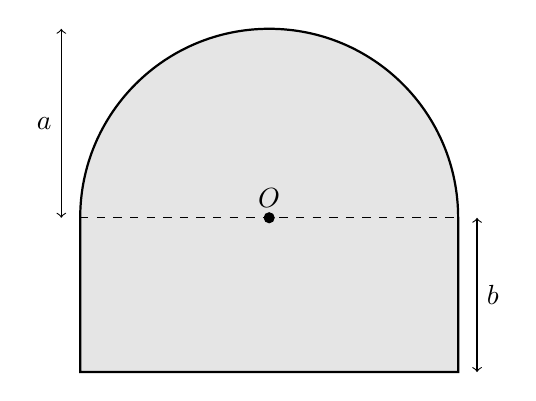
\begin{tikzpicture}[scale=1.2]
            \draw[thick, fill=gray!20] (2,0) arc (0:180:2) -- (-2,-1.633) -- (2,-1.633) -- cycle;
            \draw[dashed] (-2,0) -- (2,0);
            \filldraw (0,0) circle (1.5pt) node[above] {$O$};
            \draw[<->] (-2.2,0) -- (-2.2, 2) node[midway, left] {$a$};
            \draw[<->] (2.2,0) -- (2.2, -1.633) node[midway, right] {$b$};
        \end{tikzpicture}
    \end{center}

    若总体重心位于原点，则静矩之和必须为零：
    \begin{equation}\label{eq:center-balance}
        A_1 y_1 + A_2 y_2 = \frac{1}{2} \uppi a^2 \cdot \frac{4a}{3\uppi} + 2ab \cdot \left( -\frac{b}{2} \right) = 0.
    \end{equation}
    化简 \zcref{eq:center-balance} 得：
    \begin{equation}\label{eq:solve-b}
        \frac{2}{3} a^3 - ab^2 = 0 \implies b^2 = \frac{2}{3} a^2.
    \end{equation}
    \begin{equation}
        \boxed{b = \sqrt{\frac{2}{3}} a}
    \end{equation}
\end{solution}

\begin{problem}{三重积分重心}{Center-Of-Mass-Elliptic-Cone}
    求由曲面 $\frac{x^2}{a^2} + \frac{y^2}{b^2} = \frac{z^2}{c^2}$ 和 $z = c$ 所围成的均匀物体的重心坐标。
\end{problem}

\begin{solution}
    由几何对称性可知，均匀物体的重心位于 $z$ 轴上，即 $\bar{x} = 0, \bar{y} = 0$。

    该立体在高度 $z$ 处的截面为椭圆，其面积为：
    \begin{equation}\label{eq:area-z}
        A(z) = \uppi \cdot \left( \frac{a z}{c} \right) \cdot \left( \frac{b z}{c} \right) = \frac{\uppi ab}{c^2} z^2.
    \end{equation}
    计算体积 $V$ 及相对于 $xy$ 平面的静矩 $M_{xy}$：
    \begin{equation}\label{eq:v-and-m}
        \begin{aligned}
            V      & = \int_0^c A(z) \d z = \frac{\uppi ab}{c^2} \int_0^c z^2 \d z = \frac{1}{3} \uppi abc,     \\
            M_{xy} & = \int_0^c z A(z) \d z = \frac{\uppi ab}{c^2} \int_0^c z^3 \d z = \frac{1}{4} \uppi abc^2.
        \end{aligned}
    \end{equation}
    计算重心的 $z$ 坐标：
    \begin{equation}\label{eq:z-bar}
        \bar{z} = \frac{M_{xy}}{V} = \frac{\frac{1}{4} \uppi abc^2}{\frac{1}{3} \uppi abc} = \frac{3}{4} c.
    \end{equation}
    \begin{equation}
        \boxed{(\bar{x}, \bar{y}, \bar{z}) = \left( 0, 0, \frac{3}{4} c \right)}
    \end{equation}
\end{solution}

\begin{problem}{重心坐标计算}{Center-of-Mass-Sphere}
    设球体 $x^2 + y^2 + z^2 \leqslant 2az$ 内各点密度与各点到原点的距离成反比，求其重心坐标。
\end{problem}

\begin{solution}
    由于球体 $\Omega$ 及其密度分布关于 $z$ 轴具有旋转对称性，故其重心必在 $z$ 轴上，即 $\bar{x} = 0$、$\bar{y} = 0$。设各点密度函数为 $\rho(x, y, z) = \frac{k}{\sqrt{x^2 + y^2 + z^2}}$，其中 $k$ 为比例常数。采用球面坐标系进行计算：
    \begin{equation}
        \label{eq:Coordinate-Transformation-1}
        \begin{cases}
            x = r \sin \varphi \cos \theta, \\
            y = r \sin \varphi \sin \theta, \\
            z = r \cos \varphi.
        \end{cases}
    \end{equation}
    球体方程化为 $r \leqslant 2a \cos \varphi$，积分区域可表示为 $0 \leqslant \theta \leqslant 2\uppi$、$0 \leqslant \varphi \leqslant \frac{\uppi}{2}$、$0 \leqslant r \leqslant 2a \cos \varphi$。

    首先计算球体的总质量 $M$：
    \begin{equation}
        \label{eq:Total-Mass-1}
        \begin{aligned}
            M = \iiint_{\Omega} \rho \d V & = \int_0^{2\uppi} \d \theta \int_0^{\frac{\uppi}{2}} \d \varphi \int_0^{2a \cos \varphi} \frac{k}{r} \cdot r^2 \sin \varphi \d r \\
                                          & = 2\uppi k \int_0^{\frac{\uppi}{2}} \sin \varphi \left[ \frac{1}{2} r^2 \right]_0^{2a \cos \varphi} \d \varphi                   \\
                                          & = 4\uppi k a^2 \int_0^{\frac{\uppi}{2}} \cos^2 \varphi \sin \varphi \d \varphi                                                   \\
                                          & = \frac{4}{3} \uppi k a^2.
        \end{aligned}
    \end{equation}
    接着计算球体关于 $xy$ 平面的静矩 $M_{xy}$：
    \begin{equation}
        \label{eq:Moment-Z-1}
        \begin{aligned}
            M_{xy} = \iiint_{\Omega} z \rho \d V & = \int_0^{2\uppi} \d \theta \int_0^{\frac{\uppi}{2}} \d \varphi \int_0^{2a \cos \varphi} (r \cos \varphi) \frac{k}{r} \cdot r^2 \sin \varphi \d r \\
                                                 & = 2\uppi k \int_0^{\frac{\uppi}{2}} \sin \varphi \cos \varphi \left[ \frac{1}{3} r^3 \right]_0^{2a \cos \varphi} \d \varphi                       \\
                                                 & = \frac{16}{3} \uppi k a^3 \int_0^{\frac{\uppi}{2}} \cos^4 \varphi \sin \varphi \d \varphi                                                        \\
                                                 & = \frac{16}{15} \uppi k a^3.
        \end{aligned}
    \end{equation}
    由 \zcref{eq:Total-Mass-1} 与 \zcref{eq:Moment-Z-1} 可得重心的竖坐标为：
    \begin{equation}
        \bar{z} = \frac{M_{xy}}{M} = \frac{16/15 \uppi k a^3}{4/3 \uppi k a^2} = \frac{4}{5} a.
    \end{equation}
    综上所述，该球体的重心坐标为：
    \begin{equation}
        \boxed{(\bar{x}, \bar{y}, \bar{z}) = \left( 0, 0, \frac{4}{5} a \right)}
    \end{equation}
\end{solution}

\begin{problem}{重心与几何平衡}{Center-of-Mass-Design}
    在半径为 $a$ 的圆柱上连接一个半径为 $a$ 的半球，为了使重心正好在球心上，问圆柱之高如何？
\end{problem}

\begin{solution}
    建立空间直角坐标系，设球心位于原点 $O(0, 0, 0)$。由对称性可知重心必在轴线上。设半球位于上方 $z \in [0, a]$，其底面与高为 $h$ 的圆柱顶面相接，则圆柱占据的范围为 $z \in [-h, 0]$。

    根据质量分布均匀性，各部分质量与其体积成正比。设半球体积为 $V_1$，重心坐标为 $z_1$；圆柱体积为 $V_2$，重心坐标为 $z_2$。由几何性质可知：
    \begin{equation}
        \label{eq:Geometry-Params}
        \begin{aligned}
            V_1 & = \frac{2}{3} \uppi a^3, \quad z_1 = \frac{3}{8} a, \\
            V_2 & = \uppi a^2 h, \quad z_2 = -\frac{h}{2}.
        \end{aligned}
    \end{equation}
    欲使组合体重心落在球心处，即要求总重心坐标 $\bar{z} = 0$，根据重心公式有：
    \begin{equation}
        \bar{z} = \frac{V_1 z_1 + V_2 z_2}{V_1 + V_2} = 0 \implies V_1 z_1 + V_2 z_2 = 0.
    \end{equation}
    将 \zcref{eq:Geometry-Params} 中的参数代入上式得：
    \begin{equation}
        \left( \frac{2}{3} \uppi a^3 \right) \left( \frac{3}{8} a \right) + ( \uppi a^2 h ) \left( -\frac{h}{2} \right) = 0.
    \end{equation}
    整理方程可得：
    \begin{equation}
        \frac{1}{4} a^4 - \frac{1}{2} a^2 h^2 = 0 \implies h^2 = \frac{1}{2} a^2.
    \end{equation}
    考虑到高度 $h > 0$，求得圆柱之高为：
    \begin{equation}
        \boxed{h = \frac{\sqrt{2}}{2} a}
    \end{equation}
\end{solution}

\begin{problem}{转动惯量}{Moment-of-Inertia}
    求以下各物体的转动惯量（设 $\rho$ 为常数）：
    \begin{enumerate}
        \item 质量为 $m$，半径为 $R$ 的薄圆盘，对于：(a) 通过圆心并垂直圆盘的轴； (b) 直径。
        \item 质量为 $m$，半径为 $R$ 的球体，对于通过球心的轴线。
    \end{enumerate}
\end{problem}

\begin{solution}
    \ansitem{1}

    (a) 设圆盘面密度为 $\sigma = \frac{m}{\uppi R^2}$。在盘上取半径为 $r$、宽度为 $\d r$ 的圆环，其质量为 $\d m = \sigma \cdot 2\uppi r \d r$。
    \begin{equation}
        \label{eq:inertia-disk-z}
        \begin{aligned}
            I_z & = \int_0^R r^2 \d m                                          \\
                & = \int_0^R r^2 \cdot \frac{m}{\uppi R^2} \cdot 2\uppi r \d r \\
                & = \frac{2m}{R^2} \int_0^R r^3 \d r.
        \end{aligned}
    \end{equation}
    计算定积分可得：
    \begin{equation}
        I_z = \boxed{ \frac{1}{2} mR^2 }
    \end{equation}

    (b) 根据垂直轴定理，若 $x, y$ 轴位于圆盘平面内且互相垂直，则有 $I_z = I_x + I_y$。由对称性知 $I_x = I_y$，故
    \begin{equation}
        \label{eq:inertia-disk-x}
        I_x = \frac{1}{2} I_z.
    \end{equation}
    代入上题结果得：
    \begin{equation}
        I_x = \boxed{ \frac{1}{4} mR^2 }
    \end{equation}

    \ansitem{2}

    设球体密度为 $\rho = \frac{m}{\frac{4}{3}\uppi R^3}$。采用球坐标系，取转动轴为 $z$ 轴，则体积元 $\d V = r^2 \sin \theta \d r \d \theta \d \varphi$，点到 $z$ 轴距离为 $d = r \sin \theta$。
    \begin{equation}
        \label{eq:inertia-sphere}
        \begin{aligned}
            I_z & = \iiint_V d^2 \rho \d V                                                                                         \\
                & = \rho \int_0^{2\uppi} \d \varphi \int_0^{\uppi} \d \theta \int_0^R (r \sin \theta)^2 \cdot r^2 \sin \theta \d r \\
                & = 2\uppi \rho \left( \int_0^{\uppi} \sin^3 \theta \d \theta \right) \left( \int_0^R r^4 \d r \right).
        \end{aligned}
    \end{equation}
    其中 $\int_0^{\uppi} \sin^3 \theta \d \theta = \frac{4}{3}$，$\int_0^R r^4 \d r = \frac{R^5}{5}$，代入密度公式：
    \begin{equation}
        I_z = \frac{3m}{4\uppi R^3} \cdot 2\uppi \cdot \frac{4}{3} \cdot \frac{R^5}{5}.
    \end{equation}
    整理得：
    \begin{equation}
        I_z = \boxed{ \frac{2}{5} mR^2 }
    \end{equation}
\end{solution}

\begin{problem}{万有引力}{Gravitational-Attraction-Spherical-Cone}
    求密度为 $\rho$ 的均匀球锥体对于在其顶点为一单位质量的质点的吸引力，设球的半径为 $R$，而轴截面的扇形的角等于 $2\alpha$。
\end{problem}

\begin{solution}
    建立球坐标系，使球锥体的顶点位于原点，对称轴与 $z$ 轴重合。由于对称性，合引力 $\symbfit{F}$ 仅有 $z$ 分量。

    在球坐标下，球锥体的范围为 $0 \le r \le R$，$0 \le \theta \le \alpha$，$0 \le \varphi \le 2\uppi$。体积元 $\d m = \rho r^2 \sin \theta \d r \d \theta \d \varphi$ 对原点单位质量质点的引力 $z$ 分量为：
    \begin{equation}
        \label{eq:gravity-integral}
        \begin{aligned}
            F_z & = \iiint_V \frac{G \cdot 1 \cdot \d m}{r^2} \cos \theta                                                             \\
                & = \int_0^{2\uppi} \d \varphi \int_0^{\alpha} \d \theta \int_0^R \frac{G \rho r^2 \sin \theta}{r^2} \cos \theta \d r \\
                & = 2\uppi G \rho \int_0^{\alpha} \sin \theta \cos \theta \d \theta \int_0^R \d r.
        \end{aligned}
    \end{equation}
    计算各积分项：
    \begin{equation}
        \int_0^{\alpha} \sin \theta \cos \theta \d \theta = \left[ \frac{1}{2} \sin^2 \theta \right]_0^{\alpha} = \frac{1}{2} \sin^2 \alpha.
    \end{equation}
    代入 \zcref{eq:gravity-integral} 可得：
    \begin{equation}
        F_z = 2\uppi G \rho \cdot \frac{1}{2} \sin^2 \alpha \cdot R.
    \end{equation}
    故吸引力大小为：
    \begin{equation}
        F = \boxed{ \uppi G \rho R \sin^2 \alpha }
    \end{equation}
\end{solution}

\endinput
